\chapter{Arquitectura}

En el presente capítulo se describe la arquitectura seleccionada para la implementación del proyecto, y además se justifican las razones de su selección, comparando con otras alternativas.

Se analizaron varios tipos de arquitecturas, entre las que se encuentran:

\begin{enumerate}
    \item[$\bullet$] Arquitectura de $n$ capas ($n$-Layers)
    \item[$\bullet$] Arquitectura de cebolla (Onion Layers)
    \item[$\bullet$] Arquitectura orientada a Servicios (SOA)
    \item[$\bullet$] Arquitectura orientada a microservicios.
\end{enumerate}

Las dos últimas alternativas a pesar de ser las que mejores rendimientos en escalabilidad, desacoplamiento y extensibilidad presentan, complicarían la implementación del proyecto influyendo en el atraso de los Sprint. Lo que influye directamente en el plazo de entrega final del proyecto.

En un primer análisis cualquiera de las dos primeras alternativas parece ser idónea para este proyecto, pero se decide utilizar Onion Layers.

\section{Arquitectura seleccionada}\label{sec:arch}

La arquitectura Onion Layers no es más que una arquitectura $n$-Layers que cumple con el Principio de Inversión de Dependencias del conjunto de principios SOLID. Este principio plantea que:

\begin{enumerate}
    \item Los módulos de alto nivel no deberían depender de los módulos de bajo nivel. Ambos deberían depender de abstracciones (p.ej., interfaces).
    \item Las abstracciones no deberían depender de los detalles. Los detalles (implementaciones concretas) deben depender de abstracciones.
\end{enumerate}

En la arquitectura $n$-Layers el Principio de Inversión de Dependencias se viola pues la capa de presentación depende indirectamente de la capa de datos (la capa de presentación no funciona si no está presente la de negocio, y esta no funciona si no está presente la capa de datos), cualquier cambio que ocurra en base de datos tendrá un impacto sobre las capas superiores. Además, la capa de negocio (abstracción) no debe depender de la de datos (detalle). Los detalles deben depender de las abstracciones, como plantea el Principio de Inversión de Dependencias.

La regla principal de Onion Layers es que todo el código debe depender de las capas centrales y no de las externas.

\subsection{Diagrama de la arquitectura}\label{sec:diagrmaArch}

Se presenta en la Fig \ref{fig:onion} el diagrama de la arquitectura. Al observar los círculos concéntricos en el diagrama es que se entiende el por qué del nombre de arquitectura de cebolla.

\begin{figure}[h!]
    \centering
    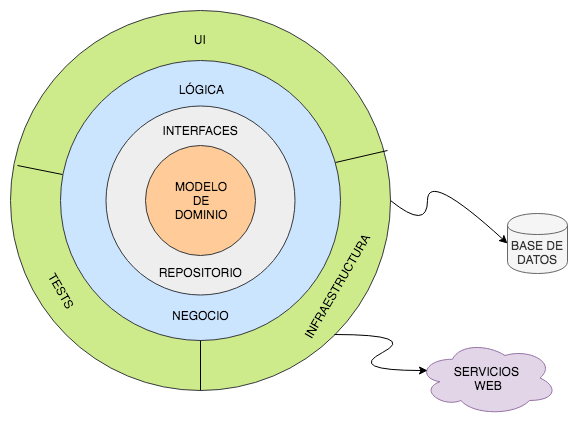
\includegraphics[width=13cm]{./chapters/img/architecture.png}

    \label{fig:onion}
    \caption{Diagrama de la Arquitectura Onion Layers}
\end{figure}

En este caso notan tres capas externas: UI, Test, Infraestructura. La UI no es más que la interfaz de usuario con la cual se comunican con la aplicación. Los test representan las pruebas que se realizan para el aseguramiento de la calidad del software en desarrollo. La infraestructura no es más que aquellos datos que son comunes a todo el sitio, por ejemplo los datos de autenticación, la base de datos y otros servicios web. Estas capas representan los detalles del software por tanto, dependen del Modelo de Dominio y el resto de capas interiores.

La finalidad de este estilo de arquitectura es poder construir aplicaciones que sean fáciles de mantener, probar y sobre todo que se encuentren desacopladas de elementos de infraestructura tales como base de datos o servicios.

\begin{enumerate}
    \item[$\bullet$] \textbf{Testeable:} Las reglas de negocio pueden ser testeadas sin necesidad de conocer la interfaz de usuario, la base de datos o algún servicio externo.
    \item[$\bullet$] \textbf{Independiente de la UI}: La interfaz de usuario puede cambiar fácilmente sin tener que afectar al resto del sistema. Un tipo de interfaz de usuario puede ser reemplazada por otra sin cambiar las reglas de negocio.
    \item[$\bullet$] \textbf{Independiente de la base de datos:} Se puede cambiar de motor de base de datos sin ningún problema. Las reglas de negocio no deben estar amarradas a esta.
    \item[$\bullet$] \textbf{Independiente de agentes externos:} Las reglas de negocio no deben saber nada que este fuera de su contexto.
\end{enumerate}